\section{复数的高次方运算}

\begin{theorem}[复数的高次方运算]
    \begin{itemize}
        \item 设 $k\in \mathbb{N}$, 则 $i^{4k}=1$, $i^{4k+1}=i$, $i^{4k+2}=-1$, $i^{4k+3}=-i$;
    \end{itemize}
\end{theorem}

\begin{example}(2023·全国乙卷)
    设 $z=\frac{2+i}{1+i^{2}+i^{5}}$, 则 $\overline{z}=($ \quad $)$
    \begin{tasks}(4)
        \task $1-2i$
        \task $1+2i$
        \task $2-i$
        \task $2+i$
    \end{tasks}
\end{example}

\vspace{4em}

\begin{example}(2023 湖北十一校联考)
    复数 $z=\frac{i^{2023}}{1-2i}$ 在复平面内所对应的点位于( \quad )
    \begin{tasks}(4)
        \task 第一象限
        \task 第二象限
        \task 第三象限
        \task 第四象限
    \end{tasks}
\end{example}

\v{4em}

\begin{example}
    $\left(\frac{1-i}{1+i}\right)^{2026}=$ \underline{\qquad}.
\end{example}

\subsection{复数的高次方的周期性}

\begin{example}
    已知复数$z$满足 $z\cdot\overline{z}=4$, 且 $z+\overline{z}+|z|=0$, 则 $z^{2022}=($ \quad $)$
    \begin{tasks}(4)
        \task 1
        \task $2^{2022}$
        \task -1
        \task $-2^{2022}$
    \end{tasks}
\end{example}

\begin{solution}
    $a+bi+a-bi+\sqrt{a^{2}+b^{2}}=0$, 所以 $2a+\sqrt{a^{2}+b^{2}}=0$.

    化简得：$2a+2=0 \Rightarrow a=-1$, 代回可求得 $b=\pm\sqrt{3}$, 所以 $z=-1\pm\sqrt{3}i$。
    \begin{itemize}
        \item 当 $z=-1+\sqrt{3}i$ 时：
              \begin{itemize}
                  \item $z=-1+\sqrt{3}i$
                  \item $z^{2}=(-1+\sqrt{3}i)^{2}=(-1)^2+2(-1)(\sqrt{3}i)+(\sqrt{3}i)^2=1-2\sqrt{3}i+3i^{2}=1-2\sqrt{3}i+3(-1)=-2-2\sqrt{3}i$
                  \item $z^{3}=z\cdot z^{2}=(-1+\sqrt{3}i)(-2-2\sqrt{3}i)=8$
                  \item 故 $z^{2022}=(z^{3})^{674}=8^{674}=(2^{3})^{674}=2^{2022}$
              \end{itemize}

        \item 当 $z=-1-\sqrt{3}i$ 时：
              \begin{itemize}
                  \item $z=-1-\sqrt{3}i$
                  \item $z^{2}=(-1-\sqrt{3}i)^2=(-1)^2+2(-1)(-\sqrt{3}i)+(-\sqrt{3}i)^2=1+2\sqrt{3}i+3i^2=1+2\sqrt{3}i+3(-1)=-2+2\sqrt{3}i$
                  \item $z^{3}=z\cdot z^{2}=(-1-\sqrt{3}i)(-2+2\sqrt{3}i)=8$
                  \item 故 $z^{2022}=(z^{3})^{674}=8^{674}=(2^{3})^{674}=2^{2022}$
              \end{itemize}
    \end{itemize}
    综上所述, $z^{2022}=2^{2022}$.
\end{solution}

\begin{tips}
    \textbf{【反思】}涉及复数的高次方计算, 往往先计算低次方, 寻找规律。
\end{tips}

\begin{example}
    已知复数 $z$ 满足 $\frac{1}{z}=\frac{1}{2}+\frac{\sqrt{3}}{2} \mathrm{i}$ ，则 $z^1, z^2, z^3, \cdots z^{2025}$ 不同的数有 （\qquad）
    \begin{tasks}(4)
        \task 6 个
        \task 4 个
        \task 2024 个
        \task 以上答案都不正确
    \end{tasks}
\end{example}

\v{8em}

\begin{example}
    已知复数 $\omega=-\frac{1}{2}-\frac{\sqrt{3}}{2} \mathrm{i}$ ， $\bar{\omega}$ 为 $\omega$ 的共轭复数，则 （\qquad）
    \begin{tasks}(2)
        \task $\omega \cdot \bar{\omega}=1$
        \task $1+\omega+\omega^2=0$
        \task $\omega+\omega^2+\omega^3+\cdots+\omega^{2024}=-1$
        \task $\omega+\omega^2+\omega^3+\cdots+\omega^{2025}=1$
    \end{tasks}
\end{example}

\v{8em}

\section{复数与曲线}

\begin{example}(2020·新课标II卷)
    设复数$z_1, z_2$满足 $|z_{1}|=|z_{2}|=2$, $z_{1}+z_{2}=\sqrt{3}+i$, 则 $|z_{1}-z_{2}|=$ \underline{\hspace{2cm}}.
\end{example}

\begin{center}
    \begin{tikzpicture}[scale=0.9]
        % 坐标轴
        \draw[->] (-2.5,0) -- (2.5,0) node[right] {$x$};
        \draw[->] (0,-2.5) -- (0,2.5) node[above] {$y$};
        \node[below left] at (0,0) {$O$};
        % 刻度
        \foreach \x in {-2,2} {
                \draw (\x,0.1) -- (\x,-0.1) node[below right] {\x};
            }
        \foreach \y in {-2,2} {
                \draw (0.1,\y) -- (-0.1,\y) node[below left] {\y};
            }
        % 圆
        \draw (0,0) circle (2);
        % 点和向量
        \coordinate (Z1) at ({sqrt(3)},-1);
        \coordinate (Z2) at (0,2);
        \coordinate (Z) at ({sqrt(3)},1);

        \fill (Z1) circle (1.5pt) node[below right] {$Z_1$};
        \fill (Z2) circle (1.5pt) node[above] {$Z_2$};
        \fill (Z) circle (1.5pt) node[above right] {$Z(\sqrt{3},1)$};

        \draw[->, blue, thick, -{Latex}] (0,0) -- (Z1);
        \draw[->, blue, thick, -{Latex}] (0,0) -- (Z2);
        \draw[->, teal, thick, -{Latex}] (0,0) -- (Z);

        % 平行四边形辅助线
        \draw[dashed, gray] (Z1) -- (Z) -- (Z2);
        % Z1Z2 向量
        \draw[->, red, thick, -{Latex}] (Z2) -- (Z1);
    \end{tikzpicture}
\end{center}

\v{2em}

\begin{example}(2022·乳山月考)
    已知复数 $z$ 满足 $|z-1|=|z-i|$, 则在复平面内$z$对应的点$Z$的轨迹为( \quad )
    \begin{tasks}(4)
        \task 直线
        \task 线段
        \task 圆
        \task 等腰三角形
    \end{tasks}
\end{example}

\v{6em}

\begin{example}
    已知 $i$ 是虚数单位, 复数 $z$ 满足 $|z|=1$, 则 $|z+1+i|$ 的最小值为( \quad )
    \begin{tasks}(4)
        \task $\sqrt{2}-1$
        \task $\sqrt{2}$
        \task $2\sqrt{2}-2$
        \task $1$
    \end{tasks}
    \begin{solution}
        设 $z=x+yi$, 则 $|z|=\sqrt{x^{2}+y^{2}}=1$, 所以 $x^{2}+y^{2}=1$.
        且 $|z+1+i|=|x+1+(y+1)i|=\sqrt{(x+1)^{2}+(y+1)^{2}}$.

        复数 $z$ 在复平面上对应的点 $Z(x,y)$ 在单位圆上运动, 式可看成点 $Z$ 与定点 $P(-1,-1)$ 的距离, 故画图来看。
        \begin{center}
            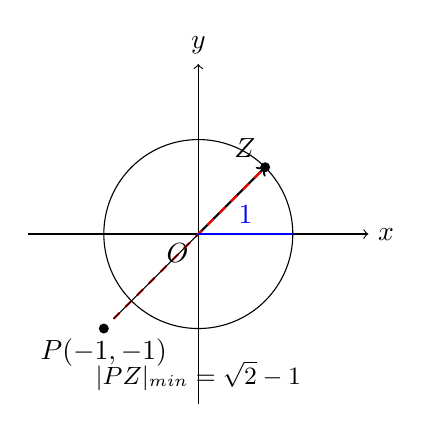
\begin{tikzpicture}[scale=1.2]
                % 坐标轴
                \draw[->] (-1.8,0) -- (1.8,0) node[right] {$x$};
                \draw[->] (0,-1.8) -- (0,1.8) node[above] {$y$};
                \node[below left] at (0,0) {$O$};
                % 单位圆
                \draw (0,0) circle (1);
                % 点 P
                \fill (-1,-1) circle (1.5pt) node[below] {$P(-1,-1)$};
                \node (P) at (-1,-1) {};
                % 点 Z (示意)
                \coordinate (Z) at ({1/sqrt(2)}, {1/sqrt(2)});
                \fill (Z) circle (1.5pt) node[above left] {$Z$};
                % 向量 OZ
                \draw[->, thick] (0,0) -- (Z);
                % 线段 PZ (最小距离)
                \draw[thick, dashed, red] (P) -- (Z);
                % 线段 OP
                \draw (0,0) -- (P);
                % 添加半径标记
                \draw[thick, blue] (0,0) -- (1,0) node[midway, above] {$1$};
                % 添加注释说明
                \node[align=left] at (0,-1.5) {\small $|PZ|_{min}=\sqrt{2}-1$};
            \end{tikzpicture}
        \end{center}
        如图, 因为 $|OP|=\sqrt{(-1)^{2}+(-1)^{2}}=\sqrt{2}$, 所以 $|PZ|_{min}=\sqrt{2}-1$。
        所以 $|z+1+i|$ 的最小值为 $\sqrt{2}-1$。
    \end{solution}
\end{example}

\vspace{6em}

\begin{example}(2022 福州模拟)
    设$i$为虚数单位, $z \in C$, 且 $(z-i)(\overline{z}+i)=1$, 则 $|z-3-5i|$ 的最大值是( \quad )
    \begin{tasks}(4)
        \task 5
        \task 6
        \task 7
        \task 8
    \end{tasks}
\end{example}

\v{10em}

\begin{example}
    已知复数 $z$ 满足 $|z-3-4 \mathrm{i}|=5$（ $i$ 为虚数单位），则复数 $z$ 在复平面上不可能位于 （\qquad）
    \begin{tasks}(4)
        \task 第一象限
        \task 第二象限
        \task 第三象限
        \task 第四象限
    \end{tasks}
\end{example}

\v{8em}

\begin{example}
    定义运算 $\left|\begin{array}{ll}a & b \\ c & d\end{array}\right|=|a d-b c|$ ，已知复数 $z=x+y \mathrm{i}(x, y \in \mathbf{R})$ ，其中 $i$ 为虚数单位，则下列说法正确的是 （\qquad）
    \begin{tasks}(1)
        \task 若复数 $z$ 满足条件 $\left|\begin{array}{ll}z & 1 \\ 2 & 1\end{array}\right|=2$ ，则复数 $z$ 对应点 $z(x, y)$ 的轨迹方程为 $(x-2)^2+y^2=2$
        \task 若复数 $z$ 满足条件 $\left|\begin{array}{ll}z & 2 \\ 3 & 1\end{array}\right|=x$ ，则复数 $z$ 对应点 $z(x, y)$ 的轨迹方程为 $y^2=12 x-36(x \geq 3)$
        \task 若复数 $z$ 满足条件 $\left|\begin{array}{ll}z & 1 \\ 3 & 2\end{array}\right|=y$ ，则复数 $z$ 对应点 $z(x, y)$ 的轨迹方程为 $4 x^2+3 y^2-12 y-9=0(y>0)$
        \task 若复数 $z$ 满足条件 $\left|\begin{array}{ll}z & \mathrm{i} \\ 1 & 2\end{array}\right|=x$ ，则复数 $z$ 对应点 $z(x, y)$ 的轨迹方程为 $3 x^2+4 y^2-4 y+1=0(x>0)$
    \end{tasks}
\end{example}

\begin{tips}
    求曲线方程一定要注意 $x$ 或 $y$ 的定义域是否符合范围的要求。
\end{tips}

\v{12em}

\begin{example}
    已知复数 $z$ 满足 $|z+1|+|z-1|=4$ ，则下列说法错误的是 （\qquad）
    \begin{tasks}(4)
        \task $|z| \leq 2$
        \task $|z-1| \geq 1$
        \task 若 $z \in \mathbf{R}$ ，则 $|z|=2$
        \task 若 $z^2 \in \mathbf{R}$ ，则 $|z|=2$
    \end{tasks}
\end{example}

\v{8em}

\begin{example}
    已知 $i$ 为虚数单位，以下选项不正确的是 （\qquad）
    \begin{tasks}(2)
        \task 若 $m, n \in \mathbf{R}$ ，则 $m+n \mathrm{i}=2+\mathrm{i}$ 的充要条件是 $m=2, n=1$
        \task 若复数 $z_1, z_2, z_3$ 满足 $z_1 z_2=z_2 z_3$ ，则 $z_1=z_3$
        \task $\mathrm{i}+\mathrm{i}^2+\mathrm{i}^3+\cdots+\mathrm{i}^{2025}=\mathrm{i}$
        \task 若复数 $z$ 满足 $|z|=1$ ，则 $|z-3+4 \mathrm{i}|$ 的最大值为 $6$
    \end{tasks}
\end{example}

\v{8em}

\begin{example}
    已知复平面上的一个动点 $Z$ 对应复数 $z$，若 $|z-4i| \leq 2$，其中 $i$ 是虚数单位，则向量 $\overrightarrow{OZ}$ 扫过的面积为 \underline{\qquad}.
\end{example}

\v{8em}

\section{复数的新定义}

\begin{example}
    （24·高一下·杨浦期末）已知 $\mathrm{i}$ 是虚数单位，设 $f(z)=\left\{\begin{array}{c}z, \operatorname{Re} z \geq 0 \\ -z, \operatorname{Re} z<0\end{array}, ~ z \in \mathrm{C}\right.$ ．
    \begin{enumerate}
        \item 已知 $z \in \mathrm{C}$ ，且 $2 f(z)+\overline{f(z)}=9-2 \mathrm{i}$ ，求 $z$ 的值；
        \item 求证：$f(z) \cdot f(\bar{z})=|z|^2$ ．
    \end{enumerate}
\end{example}

\v{12em}
